\documentclass[10pt,a4paper,fleqn,landscape]{article}

% -- Layout ----
\usepackage[top=0.25cm, bottom=0.25cm, left=0.25cm, right=0.25cm, landscape]{geometry}

% -- Titles ----
\usepackage[
  tiny,                     % text size title
  compact                   % reduce vertical space before/after title
]{titlesec}
% \titlespacing*
% \titleformat{\section}{\normalfont\Large\bfseries}{\thesection}{0em}{} % Remove space before and after section titles
% \titleformat{\subsection}{\normalfont\large\bfseries}{\thesubsection}{0em}{} % Remove space before and after subsection titles

\titlespacing*{\section}{0pt}{0pt}{0pt} % Remove space before/after section titles
\titlespacing*{\subsection}{0pt}{0pt}{0pt} % Remove space before/after subsec titles

% -- Colors ----
\usepackage[dvipsnames]{xcolor}

% -- Math ------
\usepackage{amsmath}
\usepackage{amssymb}

% -- Lists -----
\usepackage[inline]{enumitem}
\setlist{noitemsep}% Remove vspace between items
% Set vspace before and after  list environments as well as the left margin
\setlist[itemize,1]{leftmargin=*,topsep=1pt,partopsep=1pt}
\setlist[itemize,2]{leftmargin=2pt,topsep=1pt,partopsep=1pt}
\setlist[enumerate,1]{leftmargin=*,topsep=1pt,partopsep=1pt}
\setlist[enumerate,2]{leftmargin=2pt,topsep=1pt,partopsep=1pt}

% -- Code listing ---
\usepackage{listings}
\lstset{
  aboveskip=3pt,
  belowskip=3pt,
  basicstyle=\small\ttfamily,
  commentstyle=\upshape\ttfamily,
  frame=single,
  language=Haskell,
}

% Parse Trees
\usepackage{tikz}

% -- Multi Columns --
\usepackage{multicol}

% -- Global spacing settings ----
\setlength{\abovedisplayskip}{3pt}
\setlength{\belowdisplayskip}{3pt}
\setlength{\abovedisplayshortskip}{3pt}
\setlength{\belowdisplayshortskip}{3pt}
\setlength{\parindent}{0pt}
\setlength{\parskip}{0pt plus 0.5ex}

\begin{document}
% Suppress page number for all pages
\pagestyle{empty}

\begin{multicols*}{3}
\section*{Hoare logic}
% Find the \textbf{weakest precondition} (most general).\\
\textbf{Weakest} possible: \textbf{\texttt{True}} \\
\textbf{Strongest} possible: \textbf{\texttt{False}} \\
\textbf{Strong} pre/post-conditions: more \textbf{specific} (say \emph{more}) \\
\textbf{Weaker} pre/post-conditions: more \textbf{general} (say \emph{less})

\subsection*{1/6 Assignment Rule}
\subsubsection*{Question Type 1}
Given post-condition \& one single assignment, ask for pre-condition:
\(\{?\}\,S\,\{Q\}\)

For example: \(\{?\}\ i := 2 * i \{i < 6\}\)

\textbf{Solution}
\begin{enumerate}
\item \textbf{Copy} Q over to P: \(\{i_{post} < 6\}\)
\item Replace all LHS vars with RHS vars: \(\{2 * i_{orig} < 6\}\)
\item See if any math/logic equivalence (simplify P if possible): \(\{i_{orig} < 3\}\)
\end{enumerate}

\subsubsection*{Question Type 2}
Prove the given Hoare Triple: \(\{P\}\,V := E\,\{Q\}\)

For example: \(\{x > 3\}\;x:=x+2\;\{x>5\}\)
\textbf{Solution}
\begin{enumerate}
\item \textbf{Copy} Q over to P: \(\{x_{post} > 5\}\)
\item Replace all LHS vars with RHS vars: \(x_{assign}+2 > 5\}\)
\item See if any math/logic equivalence (simplify P if possible): \(\{x_{orig} > 3\}\)
\end{enumerate}



\subsection*{2/6 Pre-condition Strengthening}

Logic: \(P_{strong} \rightarrow P_{orig} \)
\begin{displaymath}
  \frac{P_{strong} \rightarrow P_{weak} \quad \{P_{weak}\}\,S\,\{Q\} } {\{P_{s}\}\,S\,\{Q\}}
\end{displaymath}

\subsection*{3/6 Post-condition Weakening}
Logic: \(Q_{orig} \rightarrow Q_{weak} \)
\begin{displaymath}
  \frac{Q_{strong}\rightarrow Q_{weak} \quad \{P\}\,S\,\{Q_{strong}\} } {\{P\}\,S\,\{Q_{w}\}}
\end{displaymath}

\subsection*{4/6 Sequencing}
\subsubsection*{Question Type}
{
  % Reducing vertical spacing
  \setlength{\abovedisplayskip}{0pt}
  \setlength{\belowdisplayskip}{3pt}
  \setlength{\abovedisplayshortskip}{0pt}
  \setlength{\belowdisplayshortskip}{3pt}

  \[\textbf{Prove:}\quad \{P\}\,S_{1};\,S_{2};\,\ldots ;\,S_{n}\,\{Q\}\]
}
\textbf{Solution} Start backwards and use Assignment Rule:
\begin{enumerate}
\item\label{step1} \textbf{Copy} \(Q_{n}\) as \(P_{n}\) for \(S_{n}\)
\item\label{step2} \textbf{Use} assignment rule and math equivalence to simplify \(P_{n}\) if possible
\item \textbf{Use} \(P_{n}\) as \(P_{n-1}\) for \(S_{n-1}\)
\item \textbf{Repeat} \ref{step1} and \ref{step2} until getting \(P_{1}\)
\item \textbf{Strengthen} precondition \(\{P\}\rightarrow \{P_{1}\}\)
\item (Optional) Sometimes need (0th/boolean) logic to simplify compound propositions.

\end{enumerate}

\subsection*{5/6 Conditionals}
\subsubsection*{Question Type}
{
  % Reducing vertical spacing
  \setlength{\abovedisplayskip}{0pt}
  \setlength{\belowdisplayskip}{3pt}
  \setlength{\abovedisplayshortskip}{0pt}
  \setlength{\belowdisplayshortskip}{3pt}

\[\textbf{Prove:}\quad \{P\}\;if\:b\:then\:S_{1}\:else\:S_{2}\;\{Q\}\]
}
\textbf{Solution} Use Conditional Rule to prove both:
\begin{description}
\item [premise1] \(\{P \land b\}\:S_{1}\:\{Q\}\)
\item [premise2] \(\{P \land \neg b\}\:S_{2}\:\{Q\}\)
\end{description}
For each premise:
\begin{enumerate}
\item\label{step1} \textbf{Use} Assignment rule to get new \(P_{assign}\)
\item\label{step2} \textbf{Use} Propositional logic, math (precondition equivalence) to \textbf{strengthen} the \(P_{assign}\) for \(P_{s}\) (which is the \(P\) needed in the premise1)
\end{enumerate}
Then \textbf{use} Conditional Rule to combine the proved premises.

\subsubsection*{Complete conditionals}
Conditionals with \texttt{else} branch are \emph{complete}.

\texttt{if b then S} $\Longleftrightarrow$ \texttt{if b then S else (do nothing)}
\begin{displaymath}
  \frac{\{P \land\; b\}\;S\{Q\} \quad \{P \land \;\neg b\}\;\texttt{(do nothing)}\;\{Q\}}{\{P\}\;if\;b\;then\;S\;\{Q\}}
\end{displaymath}
\texttt{do nothing} can be \textbf{strengthened} to sth like \verb|x := x|

\section*{DFA}
Any \(S_{c}\) has ONLY ONE transition to next \(S_{n}\)
\section*{NFA}
A \(S\) can have MANY transitions to next \(S_{n}\)
\section*{Regex}
\section*{Context-free Language (CFL)}
\newcommand{\derive}[2]{\overset{#1}{\underset{#2}{\Rightarrow}}}
\newcommand{\gor}{\;|\;}
\begin{itemize}
\item \textbf{def.
  } \(L(G) = \{w \in T^{*} \;\|\; S \derive{*}{G} w\}\)
\item \textbf{e.g.} \(L(G) = \{a^{n}b^{n} \;\|\; n \in \mathbb{N}, n \geq 1\}\)
\end{itemize}
Usually need to design the grammar (see below) for a given language
\section*{Grammar}
Design/find a grammar is to give the following:
\begin{align*}
  & G = (V,T,P,S)\left\{
    \begin{array}{l}
      V = V_{t} \cup V_{n} \\
      T = \mathsf{terminals}\; (V_{t}) \\
      P = \mathsf{productions} \\
      S = \mathsf{start \; symbol}
    \end{array}
    \right.
\end{align*}
Usually need to meet the following 6 requirements:
\begin{enumerate}
\item \(terminals\): a finite set of symbols forming the strings of the defined language
\item \(S(G) \overset{*}{\Rightarrow} w\): \(start\; symbol\) derives a \emph{w} by \(G\) in 0/more steps
\item a \emph{word}/\emph{w} contains ONLY \emph{terminals}
\item a \emph{sentential form} MUST contain 1 or more \emph{vars} (e.g. \(aSb\))
\item \emph{leftmost derivation}: always replace leftmost var by 1 of \(P\)s
\item \(A = p \in P\) that has a head of \(A\)
\end{enumerate}
\section*{Context-free Grammar (Type 2)}
\(\forall p \in P: A \rightarrow w\) where
\begin{itemize}
\item \(A \in V_{n}\) and \(w \in V^{*}\) is an arbitrary string
\item \(A\) (\textbf{left} of each \(p \in P\)) must be a \textbf{single non-terminal}
\item right-side can be anything
\item free of content, LHS can replace RHS
\end{itemize}
\section*{Regular Grammar (Type 3)}
\begin{itemize}
\item \emph{regular} means any \(p \in P\) is \emph{right-linear}/\emph{left-linear}
\item right-linear: \(A \rightarrow aB\) or \(A \rightarrow a\) or \(A \rightarrow \epsilon\) \textbf{[course focus]}
\item left-linear: \(A \rightarrow Ba\) or \(A \rightarrow a\) or \(A \rightarrow \epsilon\)
\item If \(A \derive{*}{lm} w\) AND \(A \derive{*}{lm} w\), THEN \(A \overset{*}{\Rightarrow} w\)
\item right-linear == left-linear
\item terminate with terminals or \(\epsilon\)
\end{itemize}
\section*{Common Grammar Patterns}
\begin{enumerate}
\item equal number of \(a, b\): \(T \rightarrow aTb \gor \epsilon\)
\end{enumerate}
\section*{Parse Trees}
% Minipage to show a tree in two-column
Concatenate leaves (\(V_{t}/\epsilon\)) of a parse tree \textbf{anti-clockwise}:
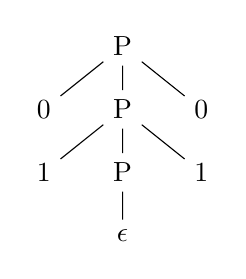
\begin{tikzpicture}[level distance=8mm,level/.style={sibling distance=10mm}]
  \node {P}
  child {node {0}}
  child {
    node {P}
    child {node {1}}
    child {
      node {P}
      child {node {\(\epsilon\)}}
    }
    child {node {1}}
  }
  child {node {0}};
\end{tikzpicture}
and get the \emph{yield} of the parse tree: \textbf{0110}
\section*{Un-ambiguous}
\emph{Ambiguous} grammar leads to \emph{un}-unique parse trees of a given string in language.  Techniques to remove ambiguity:
\begin{enumerate}
\item left/right associativity:
  \begin{itemize}
    \item[] change \(S \rightarrow S - S\) to
    \item \(S \rightarrow S - int\) [left assoc] or
    \item \(S \rightarrow int - S\) [right assoc]
  \end{itemize}
\item higher precedence: the \(V_{n}\) \textbf{closer} to \(V_{t}\) or use \verb|()|
  \begin{itemize}
    \item \(S \rightarrow S + T \gor T\) [lower]
    \item \(T \rightarrow T * \mathsf{int} \gor \mathsf{int}\) [lower]
    \end{itemize}
  \item[] \textbf{lower} level grammar productions have \textbf{higher} priority
  \item[] higher priority means the \textbf{break point} of a given string

\item Controlling \(\epsilon\):
  \begin{itemize}
    \item[] change \(S \rightarrow  \epsilon \gor (S) \gor SS\) to
    \item \(S \rightarrow \epsilon \gor T\)
    \item \(T \rightarrow TU \gor U\) and \(U \rightarrow () \gor (T)\)
    \item[] \(\epsilon\) can ONLY be derived from \(S\) and all other drvs go through T
  \end{itemize}
\end{enumerate}
\section*{PDA}
\begin{itemize}
\item defines CFG and recognizes all and only the CFGs
\item essentially an \(\epsilon\)-NFA with an additional stack
\end{itemize}
\section*{Turing Machine}

\end{multicols*}
\end{document}
